\subsection{UCW8 - Filtra classifica}

\begin{itemize}
	\item \textbf{Descrizione}: L'utente generico filtra la classifica con i risultati dei locali.
    \item \textbf{Attore primario}: Utente generico.
    \item \textbf{Precondizione}: L’utente sta visualizzando la classifica (UC3 §).
    \item \textbf{Postcondizione}: L’utente visualizza a schermo la classifica dei migliori locali gastronomici che rientrano all’interno dei filtri inseriti.
    \item \textbf{Scenario principale}: 
    \begin{enumerate}
        \item L’utente clicca il pulsante “Filtra Classifica”;
        \item L’utente applica dei filtri;
        \item L’utente clicca il pulsante “Applica Filtri”.
    \end{enumerate}

    \item \textbf{Sottocasi}:
    \begin{enumerate}
        \item Filtra per zona (UCW8.1 §);
        \item Filtra per giorno e orario di apertura (UCW8.2 §);
        \item Filtra per tipo di cucina (UCW8.3 §);
        \item Filtra per fascia di prezzo (UCW8.4 §);
        \item Filtra per punteggio (UCW8.5 §).
    \end{enumerate}

    \item \textbf{Estensioni}:
    \begin{itemize}
        \item Nel caso in cui non ci sia nemmeno un locale che rispetta i filtri applicati:
        \begin{enumerate}
            \item Viene visualizzato un messaggio che informa l’utente del fatto che nessun locale rientra nei filtri inseriti (UCE13 §);
            \item Viene fornita la possibilità di modificare i filtri.
        \end{enumerate}
    \end{itemize}
\end{itemize}

\begin{figure}[!h]
\centering
    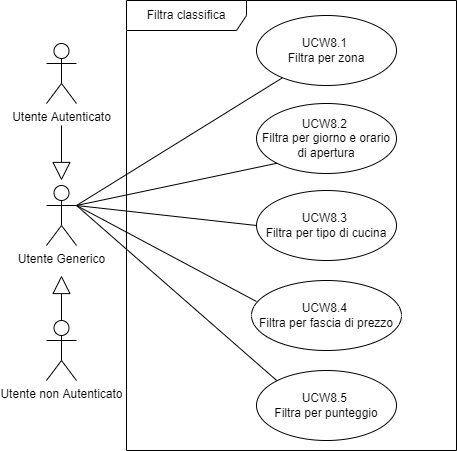
\includegraphics[scale=0.5]{UC_images/UCW8.png}
    \caption{UCW8 - Filtra classifica}
\end{figure}

\subsubsection{UCW8.1 - Filtra per zona}
\begin{itemize}
	\item \textbf{Descrizione}: L'utente generico filtra la classifica per zona.
    \item \textbf{Attore primario}: Utente generico.
    \item \textbf{Precondizione}: L’utente sta visualizzando la classifica (UC4 §) e ha premuto il pulsante “Filtra Classifica”.
    \item \textbf{Postcondizione}: Il filtro in questione viene applicato.
    \item \textbf{Scenario principale}: 
    \begin{enumerate}
        \item L’utente digita il nome di uno o più luoghi;
        \item L’utente preme il pulsante invio.
    \end{enumerate}
\end{itemize}

\subsubsection{UCW8.2 - Filtra per giorno e orario di apertura}
\begin{itemize}
	\item \textbf{Descrizione}: L'utente generico filtra la classifica per giorno e orario di apertura.
    \item \textbf{Attore primario}: Utente generico.
    \item \textbf{Precondizione}: L’utente sta visualizzando la classifica (UC4 §) e ha premuto il pulsante “filtra classifica”.
    \item \textbf{Postcondizione}: Il filtro in questione viene applicato.
    \item \textbf{Scenario principale}: 
    \begin{enumerate}
        \item L’utente seleziona uno o più giorni della settimana da un checkbox;
        \item L’utente inserisce uno o più orari;
        \item L’utente clicca il pulsante “OK”.
    \end{enumerate}
\end{itemize}

\subsubsection{UCW8.3 - Filtra per tipo di cucina}
\begin{itemize}
	\item \textbf{Descrizione}: L'utente generico filtra la classifica per tipo di cucina.
    \item \textbf{Attore primario}: Utente generico.
    \item \textbf{Precondizione}: L’utente sta visualizzando la classifica (UC4 §) e ha premuto il pulsante “Filtra Classifica”.
    \item \textbf{Postcondizione}: Il filtro in questione viene applicato.
    \item \textbf{Scenario principale}: 
    \begin{enumerate}
        \item L’utente seleziona uno o più tipi di cucina tra quelli proposti tramite un checkbox;
        \item L’utente clicca il pulsante “OK”.
    \end{enumerate}
\end{itemize}

\subsubsection{UCW8.4 - Filtra per fascia di prezzo}
\begin{itemize}
	\item \textbf{Descrizione}: L'utente generico filtra la classifica per fascia di prezzo.
    \item \textbf{Attore primario}: Utente generico.
    \item \textbf{Precondizione}: L’utente sta visualizzando la classifica (UC4 §) e ha premuto il pulsante “Filtra Classifica”.
    \item \textbf{Postcondizione}: Il filtro in questione viene applicato.
    \item \textbf{Scenario principale}: 
    \begin{enumerate}
        \item L’utente inserisce il valore minimo della fascia di prezzo;
        \item L’utente inserisce il valore massimo della fascia di prezzo;
        \item L’utente clicca il pulsante “OK”.
    \end{enumerate}
\end{itemize}

\subsubsection{UCW8.5 - Filtra per punteggio}
\begin{itemize}
	\item \textbf{Descrizione}: L'utente generico filtra la classifica per punteggio.
    \item \textbf{Attore primario}: Utente generico.
    \item \textbf{Precondizione}: L’utente sta visualizzando la classifica (UC4 §) e ha premuto il pulsante “filtra classifica”.
    \item \textbf{Postcondizione}: Il filtro in questione viene applicato.
    \item \textbf{Scenario principale}: 
    \begin{enumerate}
        \item L’utente inserisce il punteggio minimo;
        \item L’utente inserisce il punteggio massimo;
        \item L’utente clicca il pulsante “OK”.
    \end{enumerate}
\end{itemize}


%\clearpage 